\documentclass{article}

\usepackage{graphicx}
\usepackage{hyperref}


\title{Stability And Evolution Of Conway's Game Of Life}
\author{Leo BECHET  \\
Master CompuPhys (EIPHI Graduate School, Observatoire de Besançon, \\
Université de Bourgogne-Franche-Comté), 41bis Avenue de l’Observatoire, \\
BP1615, 25010 Besançon cedex,France\\
leo.bechet@edu.univ-fcomte.fr
	}

\date{\today}
% Hint: \title{what ever}, \author{who care} and \date{when ever} could stand 
% before or after the \begin{document} command 
% BUT the \maketitle command MUST come AFTER the \begin{document} command! 
\begin{document}

\maketitle


\begin{abstract}
    The analysis of cellular automaton systems, with a focus on Conway's Game of
     Life, yields significant insights into their dynamic behaviors. Our 
     examination reveals a distinct plateau in the final percentage of filled 
     cells, indicating a stable equilibrium between born, alive, and dead cells 
     within the 10\% to 70\% filling range. Interestingly, the slope of this 
     plateau remains consistent across varying resolutions, emphasizing its 
     dependency on the number of simulation steps rather than resolution. 
     Additionally, the system's evolution hints at the presence of multiple 
     stability points or a gradual convergence process. However, attempts to model 
     the plateau phase with an exponential decay curve prove inconclusive, 
     suggesting a discrepancy between fitted models and observed data. 
     Furthermore, the dynamics of the sweep's evolution exhibit intriguing 
     patterns, initially resembling a Gaussian curve before leveling off over 
     time. These findings underscore the intricate nature of cellular automaton 
     systems, highlighting the need for further research to comprehend their 
     emergent behaviors and underlying mechanisms.
\end{abstract}

\section{Introduction}
Conway's Game of Life\cite{gardner1970mathematical}, conceived by mathematician John Conway in 1970, 
is a cellular automaton operating on a grid of cells. Governed by four 
simple rules, each cell's status is determined by its neighboring cells, 
leading to a rich tapestry of patterns ranging from static formations to 
dynamic entities. Beyond its recreational appeal, the Game of Life finds 
application in scientific domains such as computer science, mathematics, 
and biology. Its enduring significance lies in its ability to stimulate 
inquiry into emergent complexity in various systems. In this article we 
will explore the evolution of the automaton for different starting
conditions. First we'll define the system, and how it works before realizing
an inital analysis of the equilibrium points of the simulation. First tests will
expose a rise in the equilibrium probability that we will try to understand, before
studying the evolution in time. Finally we will attempt to fit the time evolution of
the system to an exponential decrease. 
\paragraph{}
As of the writing of this article, there doesn't seems to have been
any work done in this area.


\section{Description of the system}
The Game Of Life is a 2D cellular automaton. It is important to note that it
has cells with only two possible state, dead or alive, charesteristic of totalistic 
automata. Totalistic cellular automata are characterized by their rules, which only 
consider the total number of live neighbors around each cell, rather than the specific 
configuration of live and dead neighbors. Our system is actually a specific set of rules
in the grand ensemble of possibilities. These automata knows as limits only the imagination of
their creator. In the case of the Game Of Life, its relevance stems from its ability to take into
consideration phenomena inherent to ecosystems, such as underpopulation, overpopulation, birth and death.

\paragraph*{Rules}
The rules of the Game Of Life are as follow \cite{catagolue} :
\begin{itemize}
    \item \textbf{Underpopulation}: A live cell with fewer than two live neighbors dies.
    \item \textbf{Survival}: A live cell with two or three live neighbors survives to the next generation.
    \item \textbf{Overpopulation}: A live cell with more than three live neighbors dies.
    \item \textbf{Reproduction}: A dead cell with exactly three live neighbors becomes a live cell.
\end{itemize}

By neighbors, we consider cells in a 3x3 grid box centered on the cell.

\paragraph*{Example of application}
Below is an example where the above ruleset is applied to a simple case.
The repetition we use here is called a "glider". It is one of the most simple
form of complex behavior that can arise from the Game Of Life.


\begin{figure}[htbp]
    \centering
    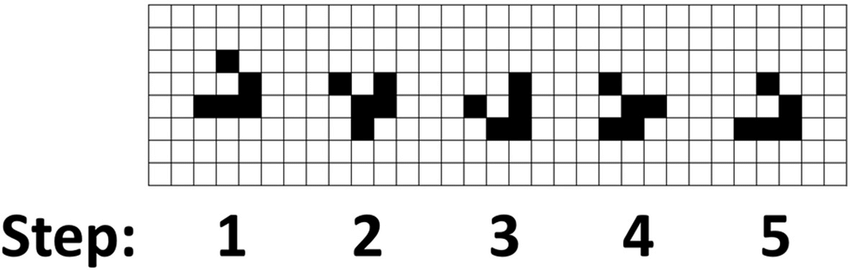
\includegraphics[width=0.8\textwidth]{res/glider.png}
    \caption{Full cycle of a glider\cite{graph}.}
    \label{fig:glider}
\end{figure}



One noteworthy characteristic of the Game Of Life ruleset is that it is Turing Complete.
Lastly, there exist multiple databases of "objects". One that we took a look at during the
writing of this article is Catagolue\cite{catagolue}

\section{Experiment context}
The focus lies on exploring the dynamics 
of Conway's Game of Life cellular automaton within a computationally 
feasible framework. The study employs a 500 by 500 grid with wrapping 
around the edges to effectively simulate an infinite grid, thus 
accommodating the inherent spatial constraints of computational 
resources. While acknowledging the potential introduction of periodic 
errors due to wrapping, the experiment adopts the perspective that in 
an infinite grid, such errors would manifest as an infinite grid can be considered as a repetition 
of an infinitely large grid. This approach allows us to 
investigate emergent phenomena and general properties of the Game of 
Life, leveraging the convenience of a finite grid while approximating 
the behavior of an infinite system. 


\section{Initial analysis}
The initial analysis phase of the experiment involves generating random 
grids with varying filling percentages, ranging from 0\% to 100\% filled, 
with each percentage representing a sweep across the spectrum of possible 
initial conditions. For each filling percentage, the simulation is run for 
1000 cycles, allowing the grid to evolve according to the rules of Conway's 
Game of Life cellular automaton. This process is repeated 10 times for 
each percentage to account for stochastic variability in the initial conditions. 
To quantify the equilibrium filling of the grid at each percentage, 20 evenly 
distributed points are selected across the simulation timeline. The final 
filled percentage is computed as the average of the last points of each of the 
10 simulations conducted for that particular percentage. These average values 
are then plotted to generate a graph illustrating the relationship between the 
initial filling percentage and the corresponding equilibrium filling state. The resulting 
graph is given in 

\begin{figure}[htbp]
    \centering
    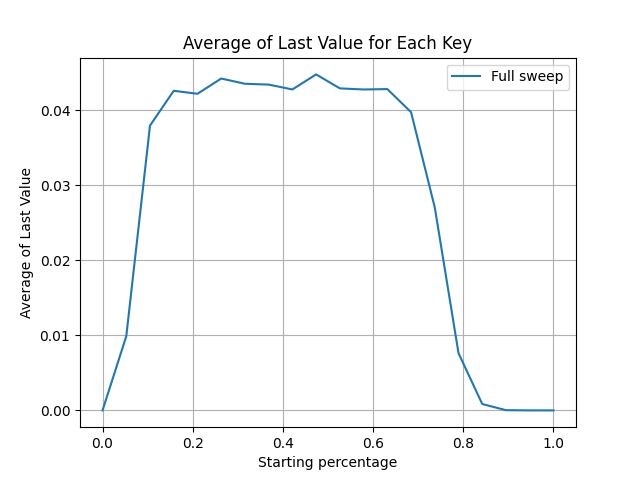
\includegraphics[width=0.8\textwidth]{res/full_start_finish.png}
    \caption{Final filling percentage for a sweep of 20 points accross 0\% to 100\% starting filling.}
    \label{fig:full}
\end{figure}

After conducting the initial simulations, it was observed in Fig \ref*{fig:full} that the final percentage 
of filled cells exhibits a non-linear trend with respect to the initial filling percentage. 
Initially, from 0\% to 10\% starting filling, the final percentage rises. 
Subsequently, between 10\% and 70\% initial filling, the final percentage stabilizes 
at around 4.5\%. Beyond 70\% initial filling, the final percentage begins to decline 
once again. This pattern suggests that the dynamics of Conway's Game of Life cellular 
automaton exhibit distinct behaviors at different ranges of initial filling percentages. 
The initial rise in final filling percentage may reflect the propagation and expansion of 
patterns from initially sparse configurations, while the subsequent stabilization could 
indicate a balance between birth and death rates of cells within moderately filled grids. 
The observed decline in final percentage at higher initial fillings may be attributed to 
increased competition and limited space for the growth and sustainability of patterns, 
leading to more frequent cell deaths. These findings highlight the intricate interplay 
between initial conditions and emergent behaviors in cellular automata systems. Further 
analysis and modeling efforts are warranted to fully elucidate the underlying mechanisms 
driving these observed phenomena. Moreover the plateau observed at 4.5\% in the final 
percentage of filled cells suggests the presence of a stable equilibrium state within 
Conway's Game of Life, indicating a critical threshold where the interplay between cell 
birth and death rates leads to sustained patterns and structures within the system.

\section{Investigating the first rise}
Due to the resolution of our graph, we do not have much precision on the first rise. Thus
we run 2 other simulations in order to increase the precision on that specific part.


\begin{figure}[htbp]
    \centering
    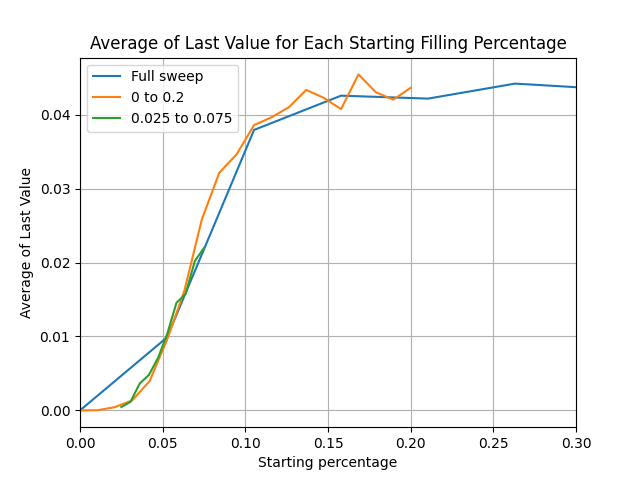
\includegraphics[width=0.8\textwidth]{res/sweep_zoom.png}
    \caption{Increased resolution sweep on the first rise.}
    \label{fig:sweep_zoom}
\end{figure}


In Fig \ref*{fig:sweep_zoom}, the medium curve in orange gives us some insight on the evolution
at low fillings. The highest resolution curve in green does not show much deviation
from the previous curve. Though we would have expected a steeper curve, it appears to slowly go up
in a quadratic fascion. We however speculate\footnote[1]{Due to the complexity of the computations, and a loss of access
to the CompuPhys server, we weren't able to investigate this supposition.} that for an infinite amount of cycle, the final sweep will be 
close to a gate function. 



\section{Evolution in time}
We consider by evolution in time, the evolution of the automaton in relation to each step.
In Fig \ref*{fig:full_evolution} we plot the previous data by averaging each the sets of 
10 runs for each percentages.

\begin{figure}[htbp]
    \centering
    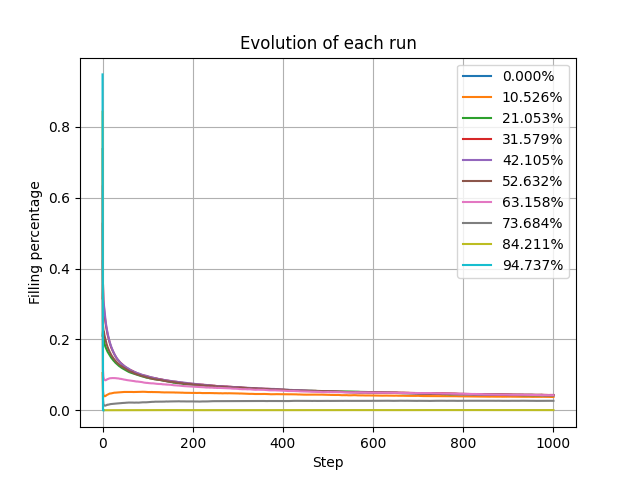
\includegraphics[width=0.8\textwidth]{res/Full_evolution.png}
    \caption{Evolution of the system for different starting fills.}
    \label{fig:full_evolution}
\end{figure}

One aspect of the graph that can be spotted is that both 0\% and 100\% curves go 
straight to a 0\% population. The simulation has checks to stop runs
once if the population reaches 0\%, thus we don't have any steps for those.
The current graph only plots half of the test fills as to not overload the graph.

Second aspect, is that we can see a heavy decrease down under 4.5\% for each percentages.
However, zooming in on the lower part of the graph, it is obvious that the evolution 
does not always follow a exponential decrease. As shown on Fig \ref*{fig:evolution_zoom}, some rise up.
This behavior is consistent for curves where the starting percentage isn't in the plateau identified
of Fig \ref*{fig:full}.

Comparing with Fig \ref*{fig:full}, curves categorized inside the plateau appear to do follow the
exponential decrease. However for the 63\% curve, it appears that it starts with an
important fall before rising up again. We do not know if that value is indeed inside
of the plateau or slitghtly off.
\begin{figure}[htbp]
    \centering
    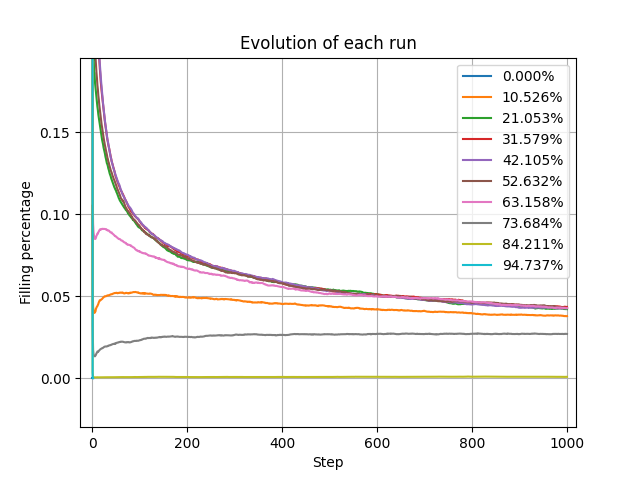
\includegraphics[width=0.8\textwidth]{res/evolution_zoom.png}
    \caption{Evolution of the system for different starting fills zoomed on the lower part.}
    \label{fig:evolution_zoom}
\end{figure}

A third aspect concerns the 84\% curve. According to Fig. \ref*{fig:full}, it is in the lower end
of the descent. Checking the evolution, it does not appear to collapse at any time and becomes rather stable.
Two scenarios can be imagined here. One would be that the evolution still tends towards the plateau,
but a very slow rate. The second is that there exists other stability point inside of the simulation.


\section{Fitting to an exponential decrease}
In order to obtain a precise value for the plateau, we propose to fit one of the central
curve to an exponential decay described in Eq. \ref*{eq:exp_decay}.

\begin{equation}
    f(x) = e^{-ax + b} + c
    \label{eq:exp_decay}
\end{equation}

\begin{figure}[htbp]
    \centering
    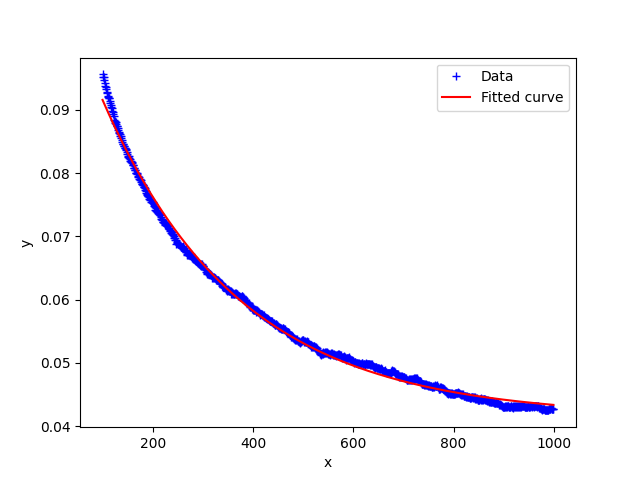
\includegraphics[width=0.8\textwidth]{res/fit.png}
    \caption{Fitting of the 42\% curve to Eq. \ref*{eq:exp_decay}}
    \label{fig:decay_fit}
\end{figure}

The following fit resulted in values of $a=0.00364699$, $b=-2.62888693$,
$c=0.04145781$. It is important to state that the first 100 points where skipped
in the fit. The comparison between the points and the fit is displayed in 
Fig \ref*{fig:decay_fit}. Fitting the whole data was not possible due to the first points.
We believe that though the exponential decay looks to be a correct fit, it
does not correspond to the right function. Fits using an inverse function were
inconclusive. From the value of $c$, we expect that the plateau is around 4.1\%
of population. It is however necessary to state that we have no proof that it is
flat, and it might aswell be bumped. The bump theory actually makes sense by allowing
descrepancies in the final value for limited number of iterations, while still leaving the 
possibility of all percentage inside the plateau to converge to the same value for an infinite number
of cycle. 
\vspace{\baselineskip}

\begin{figure}[htbp]
    \centering
    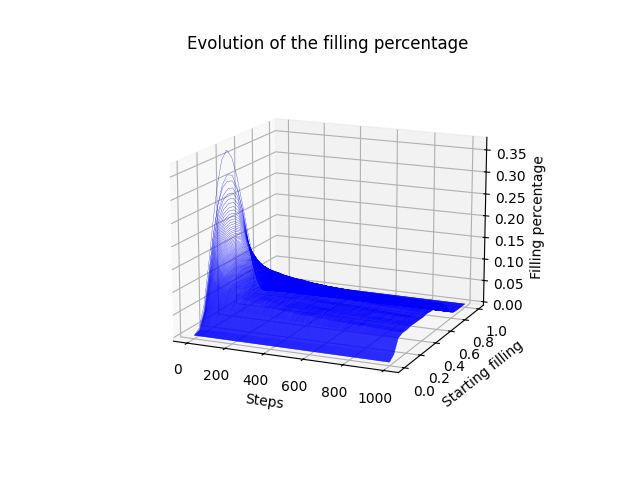
\includegraphics[width=0.8\textwidth]{res/evolution_filling.png}
    \caption{Evolution of the filling in a 3D representation.}
    \label{fig:evolution_filling}
\end{figure}

A deeper look into the evolution of the sweep curve that we introduced in Fig. \ref*{fig:full}
reveals that the original curve after 1 step looks bumpy before flattening around the middle 
(see 3D representation in Fig. \ref*{fig:evolution_filling}).
Another representation using a matplotlib generated gif is \href{https://github.com/lele394/DynamicalSystem---Game-Of-Life/blob/main/article/res/animation.gif}{available with the code}.

\section*{Conclusion}

The initial examination of the system revealed a plateau in the final percentage of filled 
cells, occurring between 10\% and 70\% starting filling. This plateau suggests the presence 
of a stable equilibrium where the balance between born, alive, and dead cells is sustainable.
Furthermore, increasing the resolution of the simulation showed that the slope of the 
plateau is not dependent on the resolution itself but rather on the number of simulation 
steps. Moreover, The evolution of the system suggests either the existence of multiple 
stability points or a slow convergence process. However, our attempts to fit a curve to 
the plateau proved inconclusive, as the fitted exponential decay curve did not align well 
with the observed data. Additionally, plotting the evolution of the sweep for each cycle 
unveiled that it initially resembled a Gaussian curve but gradually flattened over time. 
These findings underscore the complexity of cellular automaton systems and motivate further 
research into understanding their emergent behaviors and underlying mechanisms.






\begin{thebibliography}{9}
    \bibitem{gardner1970mathematical}
    Gardner, Martin. “Mathematical Games - the Fantastic Combinations of John Conway’s New Solitaire Game ‘Life’ - m. Gardner - 1970.” Universität Potsdam - Didaktik Der Informatik, Universität Potsdam , Oct. 1970, \url{ddi.cs.uni-potsdam.de/HyFISCH/Produzieren/lis_projekt/proj_gamelife/ConwayScientificAmerican.htm}. Accessed 14 May 2024.

    \bibitem{catagolue}
    Goucher, A. (2015) Game of Life Object Catalogue, Catagolue. Available at: https://catagolue.hatsya.com/ (Accessed: 18 May 2024). 

    \bibitem{graph}
    Cumming, Graeme. (2011). Introduction to Mechanistic Spatial Models for Social-Ecological Systems. DOI: 10.1007\/978\-94\-007\-0307\-0\_4.
\end{thebibliography}

\newpage


\section{Appendix}
\subsection*{Appendix A : Lyapounov exponent}
This small appendix briefly goes over the computation of the Lyapounov exponent for the system

\vspace{\baselineskip}

The Lyapounov exponent was computed using 3 distinct definition of the Tychonov 
distance. The exponent formula is 

\begin{equation}
    \frac{1}{{n+1}} \cdot \log\left(\frac{Tychonov\ distance(M_o, M_p)}{D_o}\right)
    \label{eq:Lyapounov}
\end{equation}

Where $n$ is the cycle number, $M_o$ the original matrix evolved, $M_p$ the perturbed matrix
evolved, $D_o$ the difference between the first original and first perturbed matrix, and $Tychonov\ distance$
a function giving the Tychonov distance according to the current definition. 

\paragraph{First method : Mask comparison}
The first Tychonov method counts the number of cells different between 2 grids. When plugged
in the Lyapounov exponent formula, the exponent tends towards 0.
\begin{figure}[htbp]
    \centering
    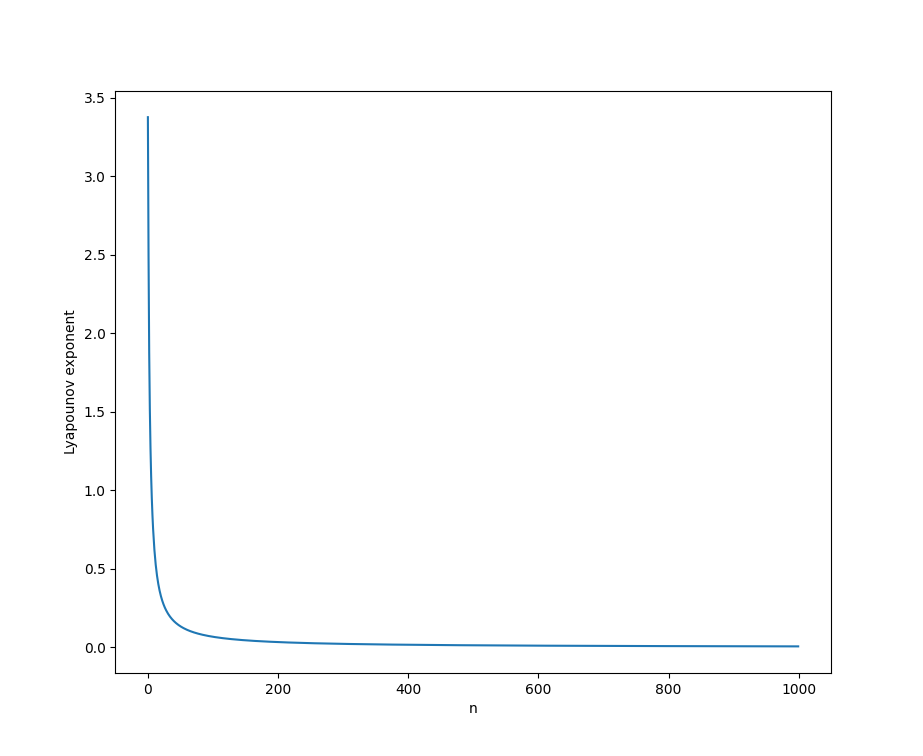
\includegraphics[width=0.8\textwidth]{res/lyapounov_1.png}
    \caption{Lyapounov exponent evolution using the mask comparison method.}
    \label{fig:lyapounov_1}
\end{figure}



\paragraph{Second method : Linear comparison}
The second Tychonov method counts the number of cells until one is different between 2 grids by 
linearising the matrices (putting rows one after the other). When plugged
in the Lyapounov exponent formula, the exponent tends towards $0^-$.
\begin{figure}[h!]
    \centering
    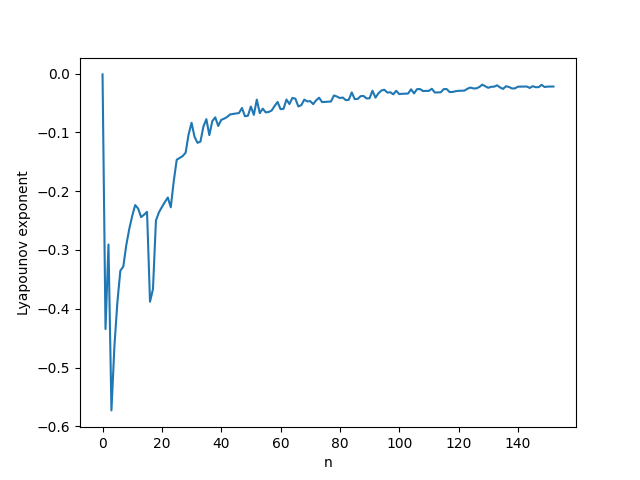
\includegraphics[width=0.7\textwidth]{res/lyapounov_2.png}
    \caption{Lyapounov exponent evolution using the linear comparison method.}
    \label{fig:lyapounov_2}
\end{figure}






\paragraph{Third method : Cirle comparison}
The Third Tychonov method counts the number of cells until one is different between 2 grids by 
starting from the center of the matrices and turning in a circular motion. When plugged
in the Lyapounov exponent formula, the exponent tends towards $0^-$.
\begin{figure}[h!]
    \centering
    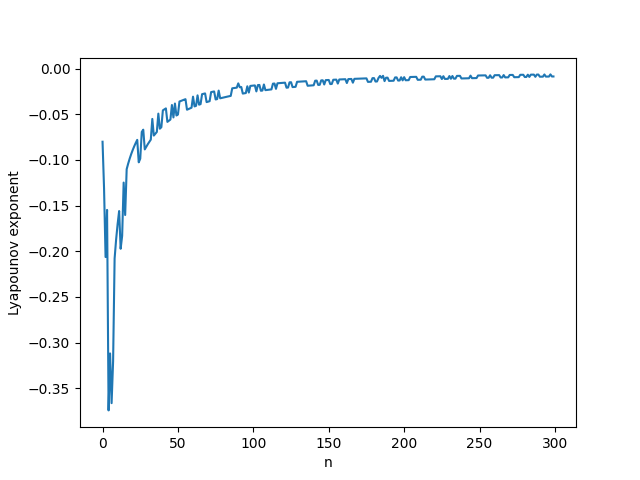
\includegraphics[width=0.7\textwidth]{res/lyapounov_3.png}
    \caption{Lyapounov exponent evolution using the circle comparison method.}
    \label{fig:lyapounov_3}
\end{figure}



\subsection*{Appendix B : Availability of the code}
The code used in this article alongside the latex code of the article iteself can be
found on the Github : \href{https://github.com/lele394/DynamicalSystem---Game-Of-Life}{github.com/lele394/DynamicalSystem---Game-Of-Life}




\end{document}